\section{Detector Characterization and Calibration}
\section{Corrections and Gating}
\section{Cross Section Calculation}
\section{Results}
\subsection{\snTwelveFour\ \el\ at 11 MeV}
\subsection{\snTwelveFour\ \el\ at 17 MeV}

Neutron energy was determined by time-of-flight, and neutron-gamma differentiation
determined by combining pulse shape discrimination (PSD) using [MODULE NAME] with
a gate on pulse height (PH). Neutron events were histogrammed by energy and the
number of counts in each bin was corrected for energy-dependent detector
efficiency [figure reference].

Initial runs were taken using (in series) a graphite, a polyethylene, and a blank
sample. A comparison of the spectra for these samples shows a peak for elastic
scattering on protons easily identifiable in the polyethylene spectrum but
absent in the graphite and blank spectra. Given the well-established n(p,p)n
cross section [cite reference] and the physical characteristics of the samples,
the ratio of incident neutron flux to the number of CMON counts can be calculated
(see [insert equation], [figure reference]). This flux-to-monitor ratio was used to normalize the
subsequent Sn sample measurements so absolute cross sections could be reported.

During data production, runs were taken in batches of three: one using 112Sn,
one using 124Sn, and one with a blank. For each angle of a given angular arm, the
efficiency-corrected histograms were normalized by the run's CMON counts,
and the relevant blank-run histogram subtracted from the isotopic-run
histograms. The major background contribution, visible in blank-run histograms
([INSERT FIGURE]), is from elastic scattering on atmospheric nitrogen
in the immediate vicinity of the sample. To calculate the cross section, the
Sn elastic peak must be integrated and the N elastic and Sn first-inelastic
peaks must be excluded. At forward angles and high neutron energies, the
difference in energy between Sn-elastic, Sn-inelastic, and N-elastic neutron
decreases and the separation between the peaks is reduced. Measurements in this
kinematic regime are the most challenging as the increased overlap between
these peaks increases the uncertainty in the Sn-elastic integral.

\subsection{Finite Size Correction}
Because the samples and angular detectors are not point-like, the exact
path of elastically-scattered neutrons is subject to a small degree of angular
uncertainty. The effect of this uncertainty is a "washing out" of measured cross
section maxima and minima with respect to the true cross section, especially in
regions where the cross section varies rapidly compared to the degree of
uncertainty. To assess the magnitude of this effect, a finite-size
simulation was prepared in which our measured cross section was assumed
to be the true cross section. In the simulation, a uniform beam of neutrons
impinged on the sample volume and was scattered into angular detectors where
hits were recorded. The resulting cross section [insert figure reference] is
thus a weighted convolution of the input cross section with the size uncertainty
of the samples and detectors. A comparison between the input and output cross
sections shows the finite-size effect is quite small in our case, much smaller
than statistical and other systematic errors. Still, to offset this effect, an
angle-dependent finite-size correction has been calculated and applied in all
results presented below.

In an idealized version of our differential cross
section measurement, the smaller the sample and neutron detectors are,
the more precisely
the angle of scattering of an incident neutron can be determined. Unfortunately,
smaller samples also reduce the rate of scattering and smaller detectors
reduce the solid angle in which scattered neutrons can be measured, both of
which reduce the number of detected neutrons and increase the statistical
uncertainty of the measurement. The experimentaler is thus responsible for applying
appropriate corrections so that reported results are apparatus-independent.

In the case of our differential cross section measurement at TUNL, the detectors'
composition, the geometry of the TOF room, and beam characteristics were
determined by the default configuration of the TUNL facility. Our samples were already
appropriately shaped for the TUNL TOF room sample suspension system and were
used for the measurement without modification. Given this configuration, we
identified two areas of concern requiring correction: the energy-dependence of
the detector efficiency ("efficiency correction") and the uncertainty in the
scattering angle due to the finite size of our sample and detectors ("finite
size correction").

\begin{figure}
    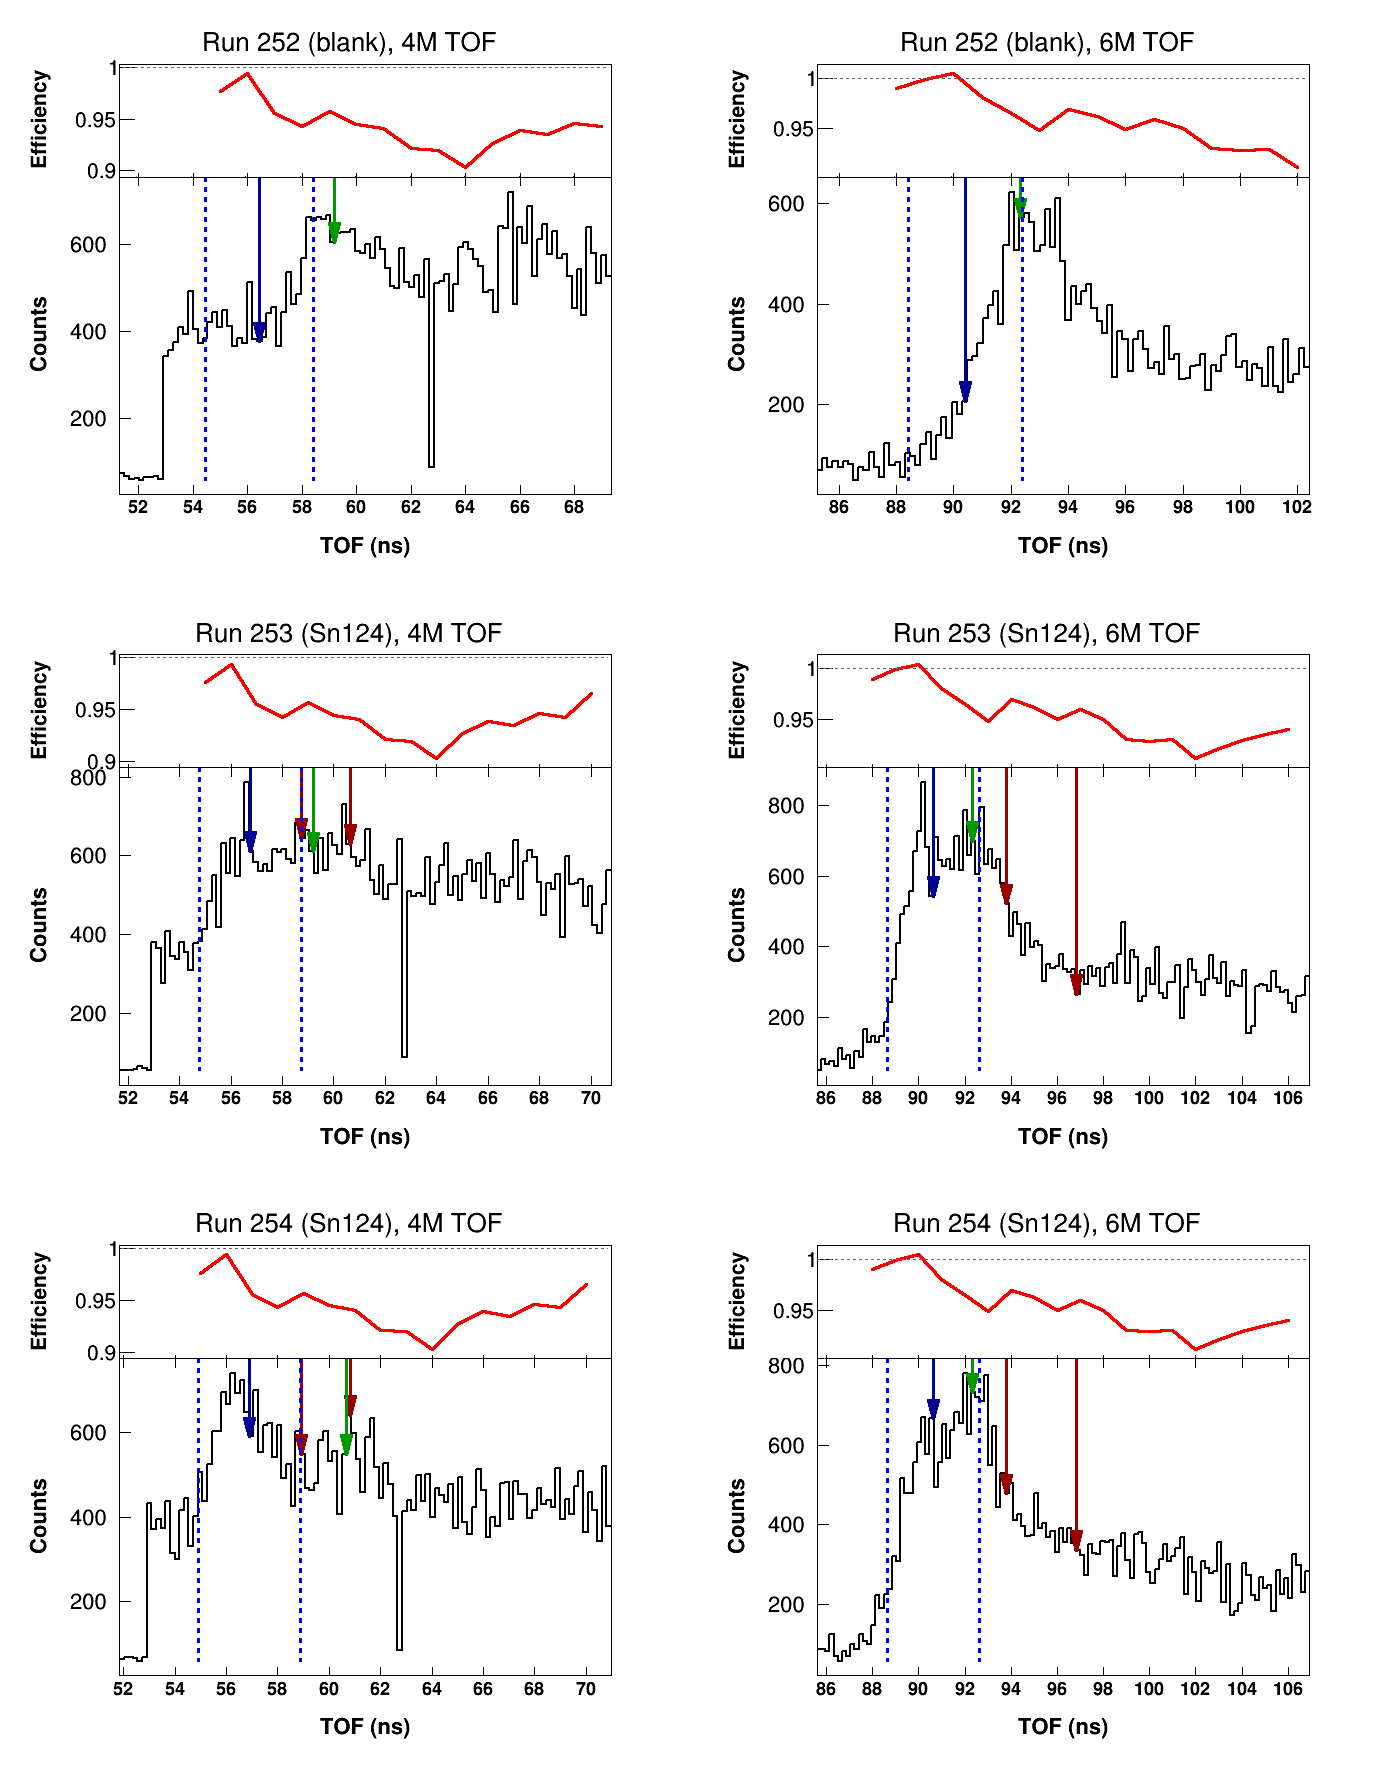
\includegraphics[width = 0.9\textwidth]{figures/tiledRunData.png}
    \caption{Typical raw event histograms showing neutron elastic scattering peak} \label{tiledRunData}
\end{figure}

Raw histograms of neutron events for several runs are shown. The
        expected location of the Sn elastic scattering peak (dark blue arrow)
        and first two inelastic scattering peaks (light blue arrows) show that
        only with the target in-beam (runs X, Y, Z) do the Sn elastic scattering
        peaks appear. For reference, the expected location of the nitrogen elastic scattering
    peak is shown in green.

\begin{figure}
    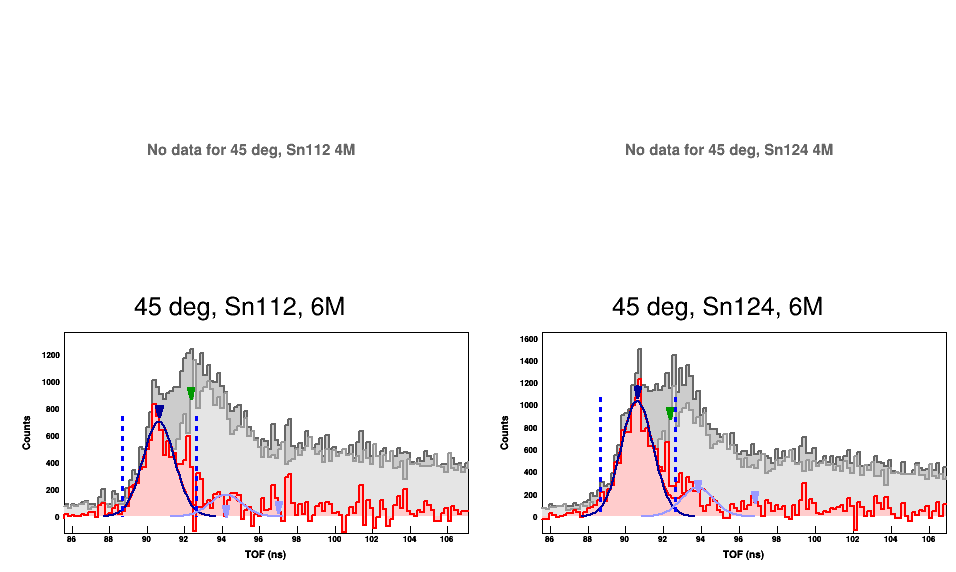
\includegraphics[width = 0.9\textwidth]{figures/tiledAngleData.png}
    \caption{Scaled event histograms showing neutron elastic scattering peak}
        \label{tiledAngleData}
\end{figure}

The background subtraction and integration procedure is shown for
        runs at 50 degrees. Sample-in-beam and sample-out-of-beam runs are
        separately summed (light gray histogram and dark gray histogram,
        respectively) and scaled by the number of monitor counts during those
        runs. The difference between those histograms (shown in red) shows a
        large elastic scattering peak at the expected TOF location (dark blue
        arrow); the first two inelastic scattering peaks (light blue arrows) are
        also shown. A double-Gaussian is fitted to the elastic and
        first-inelastic peaks and the first Gaussian integrated to recover the
        number of counts in the elastic peak. For reference, the expected location
        of the nitrogen elastic scattering peak is shown in green.

\begin{figure}
    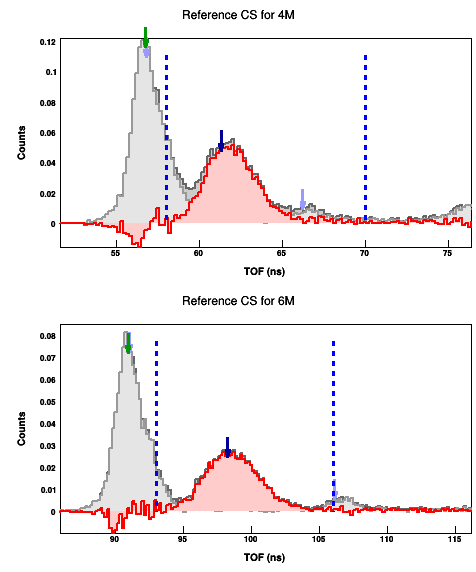
\includegraphics[width = 0.9\textwidth]{figures/polyethyleneRef.png}
    \caption{Reference run histograms showing neutron scattering on C and (CH$_{2}$)$_{n}$}
    \label{polyethyleneRef}
\end{figure}

Histograms from an example polyethylene and a graphite run (light gray
histogram and dark gray histogram, respectively) used to normalize the
cross sections. Each histogram is scaled by the number of monitor counts during
that run and their difference is taken, yielding neutrons elastically scattered
from hydrogen (red histogram). The prominent neutron-hydrogen peak is
integrated between the gates (dashed lines) and combined with the
well-established n-p cross section to create a normalization factor for
the Sn runs. The neutron TOFs for scattering from carbon (elastically at the dark blue
arrow, to the first excited state of carbon at the light blue arrow)
and nitrogen (elastically at the green arrow) are indicated.

\begin{figure}[ht]
    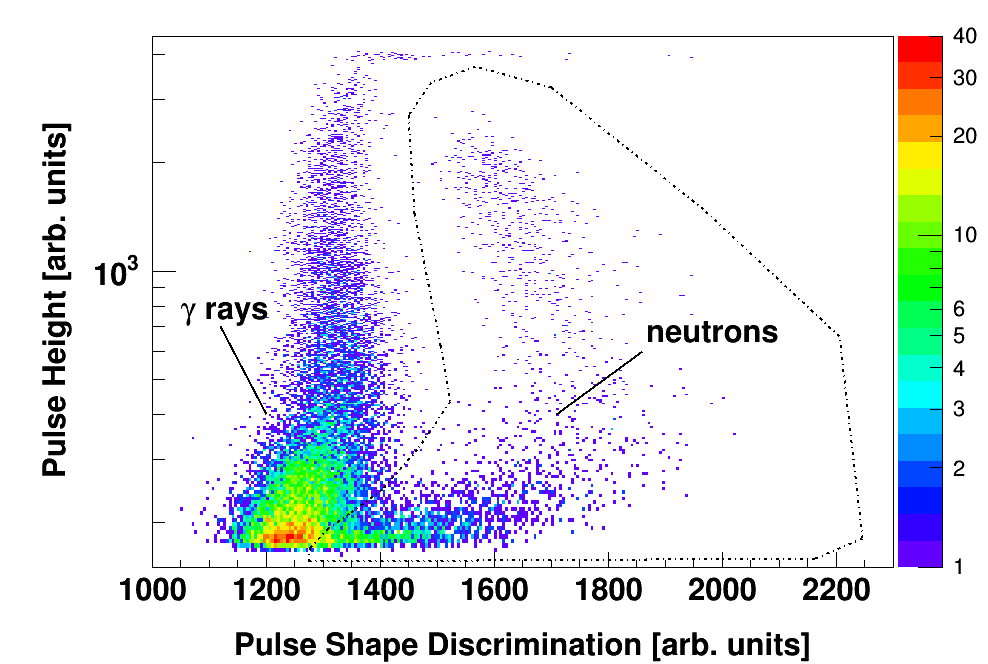
\includegraphics[width=0.9\textwidth]{figures/PHPSDPlot.png}
    \caption{The pulse height (PH) versus pulse-shape-discrimination (PSD) for
    events of a typical run.}
    \label{PHPSDPlot}
\end{figure}

Efficiency correction was straightforward: the detector response with respect to
neutron energy had already been tabulated by TUNL staff. Accordingly, we
adjusted the number of counts in each bin of our detector histograms according
to the bin's energy (shown in Fig. [X]). To understand finite-size effects, a
Monte Carlo simulation was developed in which the sample and detector geometry
could be varied and the effect on the cross section visualized. As illustrated
in Fig. [X], in an experiment with point-like detectors and
samples, the scattering angle for a given configuration can be exactly
determined. In a realistic experiment, however, the finite size of the sample
introduces uncertainty in the location of the scattering vertex and the finite size of the
detector introduces uncertainty in the location of the detection vertex. Consequently, the cross
section calculated for a given angle also includes unwanted contributions
from nearby angles; correcting for this effect is essentially a "deconvolution"
of the scattering trajectories with respect to the sample and detector geometry.

For simplicity, the simulation was purely geometric - no nuclear physics or
energy-dependence was included. For each Monte Carlo iteration, the beam was
assumed to uniformly illuminate
the sample from one direction so that the scattering vertex was randomly
distributed within the sample volume. At the scattering vertex, a neutron
trajectory was selected by randomly sampling an "input cross section" as a
probability mass function, thus weighting the neutron scattering angles by the
input cross section.  Once the trajectory was known, each detector's location
and orientation was used to calculate the point of intersection in the plane of each detector. If the
intersection fell within the detector's face, the detector registered a hit.
Finally, the "output cross section" (that is, the result of the simulation)
was calculated by normalizing the number of counts registered in each detector
over the total number of iterations and the fraction of the total solid angle
subtended by said detector.

The results of the simulation are visible in Fig. [X]. For the sample and
detector sizes actually used in the experiment, the deviation between the input
and output cross sections is <1\% over all angles. When exaggerated sizes for the
sample and detectors are used, the finite-size effect is visible as a "washing
out" of minima and maxima in regions where the cross section varies rapidly with
angle. To calculate a correction factor for our results, we divided the simulation's
input cross section by the output cross section for each angle and multiplied our
experimental results by this factor. In principle, this procedure to generate
the correction should be repeated iteratively because the correction changes the input distribution 
used for the simulation itself, but in practice the correction is so small
that no further iteration is required.

Absolute cross sections 

\begin{figure}
    \begin{center}
        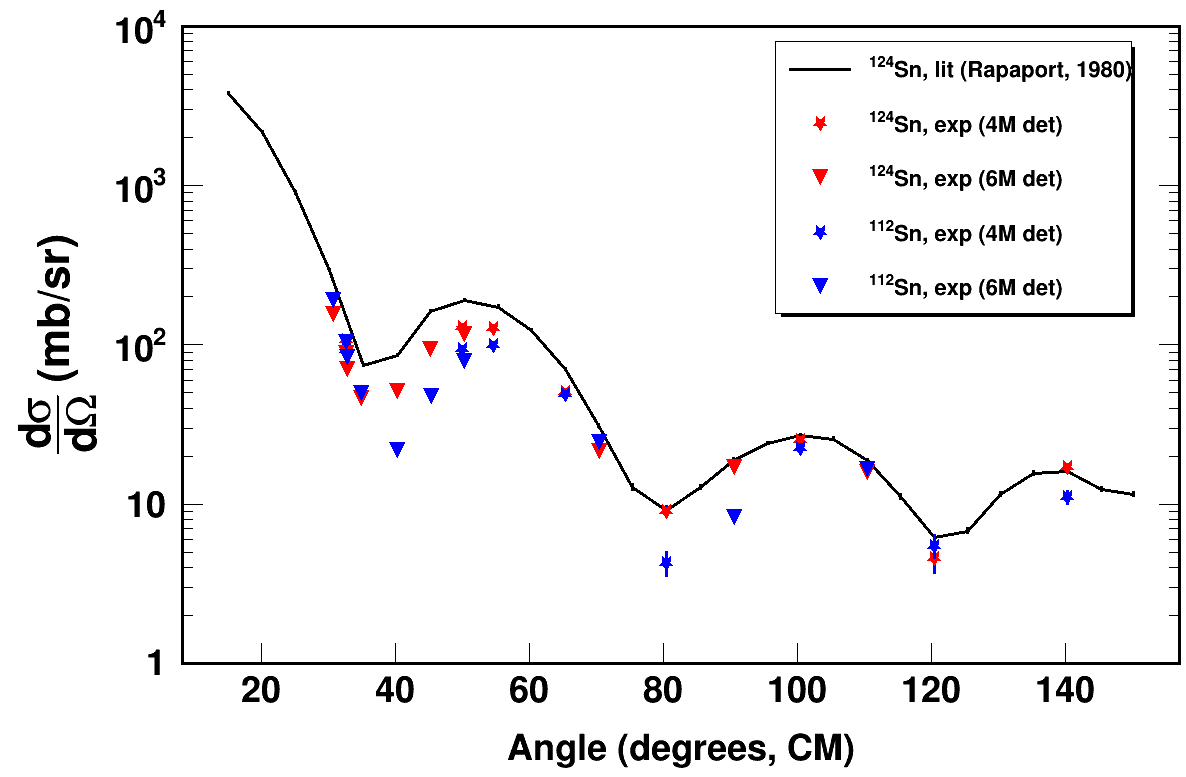
\includegraphics[width = 0.9\textwidth]{figures/neutronECS_Sn_11MeV.png}
        \caption{Neutron \el cross sections on $^{112,124}$Sn at 11
    MeV: our results and literature data}
    \label{SnECS_11MeV}
\end{center}
\end{figure}

\begin{figure}
    \begin{center}
        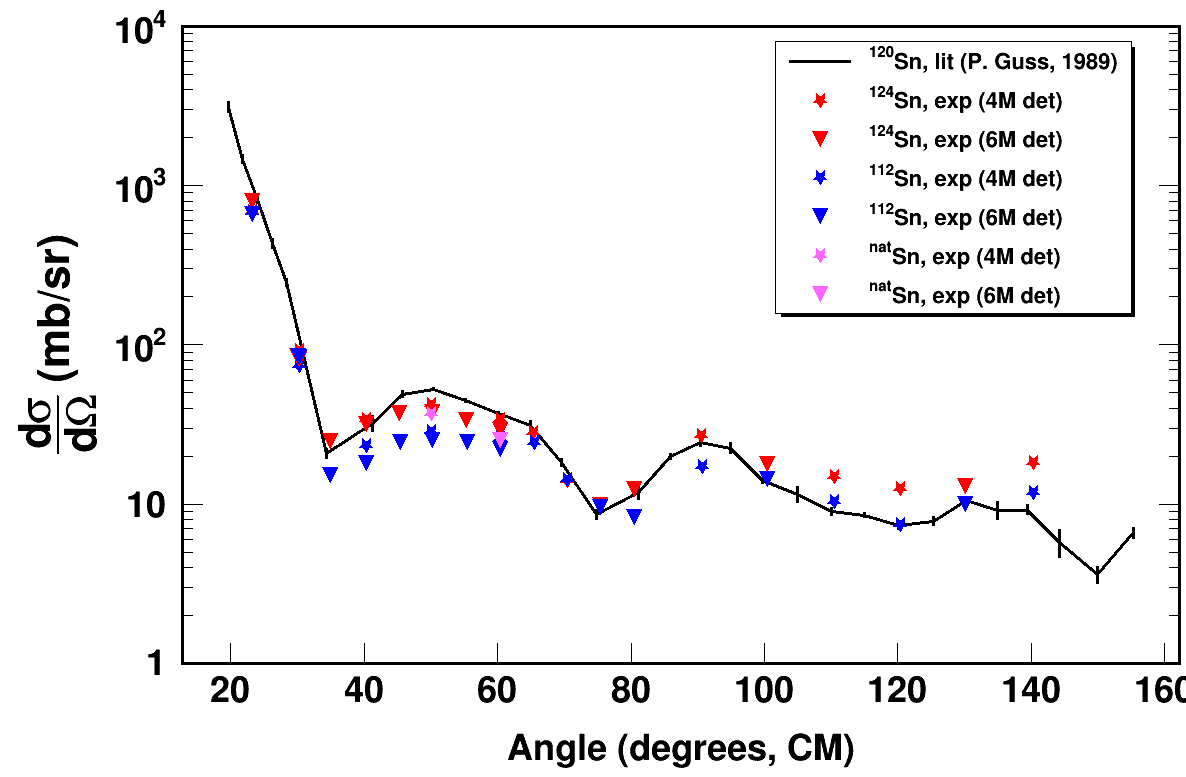
\includegraphics[width = 0.9\textwidth]{figures/neutronECS_Sn_17MeV.png}
        \caption{Neutron \el cross sections on $^{112,nat,124}$Sn at 17
    MeV: our results and literature data} \label{SnECS_17MeV}
\end{center}
\end{figure}

\afterpage{\clearpage}
